\section{Implementation of \hpl}
\label{sec:implementation}


\begin{figure*}[bth]
\begin{center}
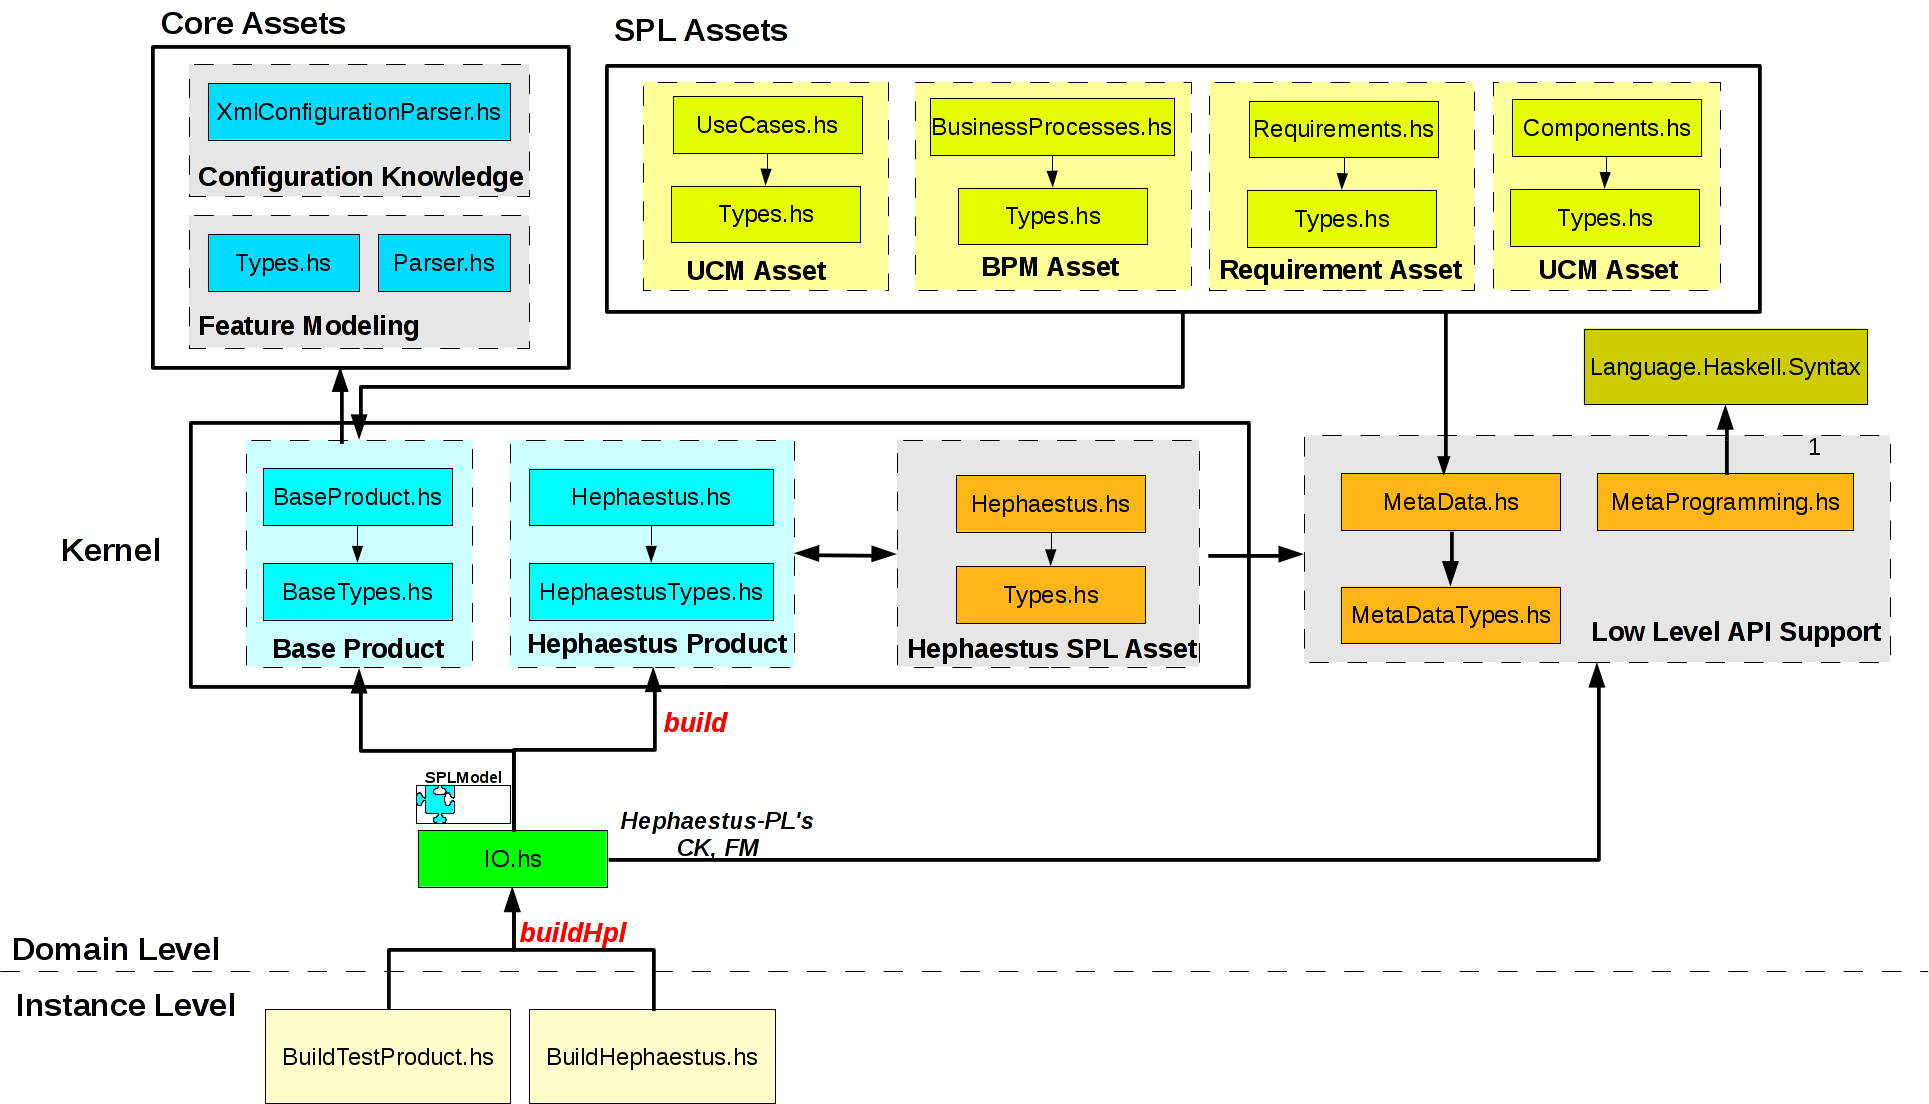
\includegraphics[scale=0.35]{imagens/modules-hpl.png}
\end{center}
\caption{Hephaestus-PL's modules dependency}
\label{fig:modules-hpl}
\end{figure*}


%\subsection{Objective of the experiment}

%The objective was to understand whether a) Haskell metaprogramming techniques can be used to obtain instances of Hephaestus that cover selected variations of assets, e.g., use cases and business processes, and b) such a metaprogramming approach can be provided in a way that the Hephaestus product-line infrastructure is applied to itself.

%\subsection{Summary of the results}

%Subject to a number of simplifying assumptions, the experiment was successfully completed. One simplification concerns the assets in scope. We used mockups as opposed to the actual implementations in Hephaestus. If we were to use the actual implementations, the relevant modules may require some changes. Another simplification concerns the feature model of Hephaestus. We only consider the OR feature for the different assets.

In this section we present the details of the implementation of \hpl's architecture shown in the Figure~\ref{fig:architecture-hpl} in terms of modules e their dependencies, as depicted in Figure~\ref{fig:modules-hpl}.
The dotted line comprises the modules which compose each of the main elements in the \hpl's architecture, i.e., the \texttt{BaseProduct.hs} and \texttt{BaseTypes.hs} modules are the \textit{Base Product} of the \hpl's Kernel.
We present the domain level's modules which support the generation of new \hpl{} intances and the instance level's modules which were developed to test \hpl{} with a selected feature configuration. Besides that, we present the metaprogramming operations which implement the transformations in Haskell code of a \textit{Base Product} of the \hp{} instance.
The source code of \hpl{} is publicly\footnote{https://gitorious.org/hephaestus-pl/hephaestus-pl} available.


\subsection{Modules and Dependencies}

At the domain level, the \texttt{IO.hs} module contains the \texttt{buildHpl} function which represents the interface to the \hpl{}'s instance level. This function is the initial point for the generation of a new \hpl{} instance by the \hpl{}'s product derivation process.  
The \texttt{buildHpl} function receives a feature configuration of \hpl{}'s FM as input and prepares the environment to execute the generation of \hpl{} instance (guided by \texttt{build} function of \textit{\hp{} Product}). 
The inputs to the derivation process of \hpl{} are four: a instance of the \texttt{SPLModel} data type, a valid feature configuration and the \hpl's FM and CK.
In this context, the instance of the \texttt{SPLModel} data type wraps the \hp{} asset, i.e., the physical modules of the \textit{\hpl{} base product} are inserted into an instance of \texttt{HephastusModel} data type that represents the abstract type of \hp{} asset and it is wrapped into an \texttt{SPLModel} data type. 
Besides, the derivation process of \hpl{} needs the \hpl{}'s feature modeling and configuration knowledge
%has the goal of preparing the elements (\texttt{SPLModel} data type, feature modeling and configuration knowledge) of \hp{} 
to execute the \texttt{build} function of the \textit{\hp{} Product} that controls the generation of the new \hpl's instance. 
The \hpl's FM and CK are contained into \texttt{MetaData.hs} module. Then, 
%Thus, are selected the \textit{Base Product's} modules which represent the \texttt{HephastusModel} data type and are inserted into \texttt{SPLModel} data type and are selected the \hpl's FM and CK contained into \texttt{MetaData.hs} module to call 
the \texttt{build} function contained into \texttt{\hp.hs} module (\textit{\hp{} Product}) is executed and returns the new \hpl{} tool instance. 
Therefore, the \texttt{IO.hs} module depends of \textit{Base Product's} modules, \textit{\hp{} Product's} modules and \texttt{MetaData.hs} module, as shows the Figure~\ref{fig:modules-hpl}.

The \textit{\hp{} Product's} modules depend strongly on \textit{\hp{} SPL Asset's} modules that implement the \texttt{HephaestusModel} and \texttt{HephaestusTransformation} data types and \texttt{transformHpl} function, i.e., the \texttt{build} function evaluates the CK and calls the \texttt{transform} function defined in the same \hp.hs module into \textit{\hp{} Product} that executes the \texttt{transformHpl} function into \hp.hs module of \textit{ \hp{} SPL Asset} to solve the \hpl{} transformation.

The \texttt{MetaData.hs}, \texttt{MetaDataTypes.hs} and \texttt{MetaProgramming.hs} modules comprise the group called \textit{Low Level API Support} that implement the metaprogramming operations to solve the variation points in \textit{Base Product's} modules. The \texttt{MetaProgramming.hs} module depends the Language.Haskell.Syntax package.

The \textit{SPL Assets} are composed by pairs of modules: the \texttt{Types.hs} module which defines the algebraic data types of the asset to insert into \texttt{SPLModel} and \texttt{InstanceModel} data types of \hpl{} instance and defines the data types which are used as constructors into \texttt{TransformationModel} and \texttt{ExportModel} data types of \texttt{BaseTypes.hs} module. 
Besides, another module (\texttt{assetName.hs}) of each group in \textit{SPL Assets} defines the functions which are used into \texttt{transform}, \texttt{mkEmptyInstance} and \texttt{export} functions of \texttt{BaseProduct.hs} module. Thus, the \textit{SPL Assets} modules depend the \textit{Base Product's} modules.

Finally, we have the \textit{Core Assets'} modules (FM and CK) that are imported by \textit{Base Product's} modules.



\subsection{Description of the Transformational Approach}

The underlying hypothesis is that certain key types and functionality of any specific Hephaestus instance can be derived by metaprogramming. To this end, we consider an \texttt{Base Product} from which to build ``\hpl{} products''. All products are expected to define \texttt{SPLModel}, \texttt{InstanceModel}, \texttt{ConfigurationKnowledge}, \texttt{TransformationModel}, \texttt{ExportModel}, a transformation function \texttt{transform}, a output format function \texttt{export} and \texttt{main} function that controls the generation the product instances.

All forms of assets are hence provided in a form that they can contribution to the above-mentioned entities as presented in SPL Asset block in Figure~\ref{fig:modules-hpl}. We use metaprogramming operators that build the product's entities (say, types and functions) from the corresponding parts of the asset-related modules by adding parts incrementally to the base product.

Because of the objective of self-application of Hephaestus (bootstrapping design principle), the above-mentioned transformational approach is actually packaged as another kind of asset: Hephaestus SPL Asset. That is, the construction of any specific Hephaestus instance is controlled by a feature configuration relative to \hpl's feature model and the corresponding configuration knowledge as presented in module \texttt{MetaData.hs}.


\subsection{Metaprogramming Operations} \label{sec:metaprogrammingOperations}

\begin{table}[h]
%\begin{tabular}{||l||l||}
\begin{tabular}{ | l | p{7cm} |}
  \hline
  \textbf{\hpl{} Transformations}            & \textbf{Metaprogramming Operations}  \\  \hline
  \multirow {9} {*} {\textit{SelectAsset assetName}} & addUpdateCase \\ \cline{2-2}
                                             & initializeFieldWithFun \\ \cline{2-2}
                                             & addImportDecl (4x) \\ \cline{2-2}
                                             & addLetInstruction \\ \cline{2-2}
                                             & addGeneratorInstruction \\ \cline{2-2}
                                             & initializeField  \\ \cline{2-2}
                                             & addField (2x)  \\ \cline{2-2}
                                             & addConstructor  \\ \cline{2-2}
                                             & addUpdateCaseList \\  \hline
 \multirow {4} {*} {\textit{SelectExport assetFormat}} & addUpdateCase  \\ \cline{2-2}
                                               & addImportDecl  \\ \cline{2-2}
                                               & addConstructor \\ \cline{2-2}
                                               & addListElem \\ \hline
 \multirow {2} {*} {\textit{SelectBaseProduct}} & setModuleName (2x)  \\ \cline{2-2}
                                     & removeImportDecl \\ \hline
 \textit{BindProductName}            & setModuleName (2x)  \\ \hline
 \textit{RemoveProductMainFunction}  & removeFunction \\ \hline
 \multirow {3} {*} {\textit{SelectCKParser}}  & addImportDecl \\ \cline{2-2}
                                     & addGeneratorInstruction  \\ \cline{2-2}
                                     & addLetInstruction (2x) \\ \hline
\end{tabular}
\caption{Mapping of \hpl{} transformations into metaprogramming operations}
\label{tab:map-transformations-hpl}
\end{table}


%  \multirow {\textit{SelectAsset assetName}} & addUpdateCase & extends \textit{transform} function \\ \cline{2-3}
% & initializeFieldWithFun & initialize \textit{InstanceModel} with empty asset \\ \cline{2-3}
% & addImportDecl & import modules data types, transformations and parser of asset \\ \cline{2-3}
% & addLetInstruction & update \textit{main} function ... \\ \cline{2-3}
% & addInstructionGenerator & insert asset's parser function in \textit{main} function \\ \cline{2-3}
% & initializeField & update SPLModel data type in \textit{main} function \\ \cline{2-3}
% & addField & insert asset data type in \textit{SPLModel} and \textit{InstanceModel} data types \\ \cline{2-3}
% & addConstructor & insert asset transformation data type in \textit{TransformatonModel} data type \\ \cline{2-3}
% & addParserCKList & insert asset transformation names in \textit{xml2Transformation} function \\  \hline
% \multirow {\textit{SelectExport assetFormat}} & addUpdateCase & extends \textit{export} function \\ \cline{2-3}
% & addImportDecl & import asset output format module \\ \cline{2-3}
% & addConstructorWithoutArgs & insert asset output format data type in \textit{ExportModel} data type \\ \cline{2-3}
% & addElemList & insert asset output format data type in \textit{lstExport} list \\ \hline
% \textit{SelectBaseProduct}} & setModuleName & rename the \hpl{} instance module from "BasicProduct" to "Test" \\ \cline{2-3}
% & removeImportDecl & \\ remove the line \texttt{import HplProducts.EmptyTypes} from \hpl{} instance module \cline{2-3}
% & addImportDecl & \\ \cline{2-3}
% & addInstructionGenerator & \\ \hline
% \textit{BindProductName}} & setModuleName &  \\ \hline


The required metaprogramming operations are of different complexity as implemented in \texttt{MetaProgramming.hs} module. We begin with the simpler operations. There is an operation \texttt{setModuleName} to modify the module name so that the module of the base product can be renamed into a module for the emerging product, say \hp{} instance. This operation is performed on the \texttt{SelectBaseProduct} and \texttt{BindProductName} transformations.
There is an operation \texttt{addImportDecl} to add an import declaration to the main module of the emerging product; this operation is needed to incorporate any additional kind of asset. This operation is performed on the \texttt{SelectCKParser} transformation to add an import declaration to CK parser (\texttt{CK.Parsers.XML.XmlConfigurationParser} module); on the \texttt{SelectAsset} transformation to add import declarations to incorporate the asset modules (algebraic data types, transformations, parser and output format) and the data types module of emerging product.
There is an operation \texttt{addField} to extend a given record type with a field; this operation is needed in the extension of Hephaestus' data types \texttt{SPLModel} and \texttt{InstanceModel}.
There is also an operation \texttt{addConstructor} to extend a given algebraic data type with a constructor declaration besides to remove the constructor declaration not used, i.e., \texttt{UndefinedTransformation} constructor; this operation is needed for assembling Hephaestus' data type \texttt{TransformationModel} for transformations on possibly different forms of assets. We note here that \texttt{addConstructor} is deliberately limited to only support the addition of a constructor with a single constructor component and to actually reuse that component's specified type for the constructor's name.
Therefore, we defined a similar operation \texttt{addConstructorWithoutArgs} to extend the Hephaestus' data type \texttt{ExportModel} for different asset output formats. In this case, the \texttt{addConstructorWithoutArgs} only supports the addition of a constructor's name without components. We also remove the variation point declaration \texttt{UndefinedExport} in this operation.
The operation \texttt{addListElem} adds into \texttt{lstExport} list the constructors of the Hephaestus' data type \texttt{ExportModel}.

The addition of fields and constructors is relatively straightforward at the type level, but we need additional, non-trivial operations that transform functions that readily use the affected types. There are the operations \texttt{initializeField} and \texttt{initializeFieldWithFun} which modify all expressions for record construction for a given record type such that in the first case a given field is initialized by a constant (say, a variable name or a function name with assumed zero arity) and in the second case a given field is initialized by a function name with assumed one arity, i.e., the empty asset function that receives the asset data type as input parameter. Other forms of reaction to added fields are conceivable, but the given form turned out to be sufficient in the experiment.
There is also an operation \texttt{addUpdateCase} which extends function definitions by a case in reply to a previously added constructor. Different forms of adding cases are conceivable. The following, non-trivial form was required in the experiment.

Addition of a constructor is needed for \texttt{TransformationModel}, which in turn is to be used in a \emph{transform} function that essentially interprets transformation models (`terms'). The type of the function is this:

\begin{lstlisting}
transform :: TransformationModel
          -> SPLModel
          -> InstanceModel
          -> InstanceModel
\end{lstlisting}

The idea is here that the function perhaps case discrimination on the \emph{first} argument and essentially delegates to a more specific transformation function that readily handles the given transformation on the further arguments at hand. An additional complication arises from the fact that the more specific transformation function would not be able to operate on the composed types \texttt{SPLModel} and \texttt{InstanceModel}. For example, consider a Hephaestus instance that should support use cases and business processes. Then, the following \texttt{transform} function has to be synthesized:

\begin{lstlisting}
transform (UseCaseTransformation x0) x1 x2 = transformUcm  x0 x1 x2
transform (BusinessProcessTransformation x0) x1 x2 = transformBpm  x0 x1 x2
\end{lstlisting}

Hence, the  operation \texttt{addUpdateCase} must add cases such that indeed case discrimination is performed on the first argument and the last two arguments are defined by \texttt{x1} and \texttt{x2} variables when being passed to the function on the RHS.
A similar operation to \texttt{addUpdateCase} was defined to extend the \texttt{export} function definition by a case in reply to a previously added constructor into \texttt{ExportModel} data type. The type of the function is this:

\begin{lstlisting}
export :: ExportModel -> FilePath -> InstanceModel -> IO ()
\end{lstlisting}

For example, consider a Hephaestus instance that should support use cases and business processes in xml format. Then, the following \texttt{export} function has to be synthesized:

\begin{lstlisting}
export :: ExportModel -> FilePath -> InstanceModel -> IO ()
export (ExportUcmXML) x1 x2  = exportUcmToXML (x1 ++ ".xml") (ucm x2)
export (ExportBpmXML) x1 x2  = exportBpmToXML (x1 ++ ".xml") (bpm x2)
\end{lstlisting}

The extension of the \texttt{xml2Transformation} function is also done with the \texttt{addUpdateCase} operation applied in a list of cases of transformations supported by CK for the emerging \hpl{} product.


Moreover, we defined two new operations to extend the \texttt{main} function into a module for the emerging product, they are \texttt{addLetInstruction} and \texttt{addGeneratorInstruction}. The first is used to add  \texttt{let} sentences in the \texttt{main} function to recover the asset spl and to execute the parser function and moving the asset spl into \hpl's instance. The second operation \texttt{addGeneratorInstruction} is used to add instructions about asset and CK parsers into module for the emerging product.
The operation \texttt{addLetInstruction} adds the instruction \texttt{let product = build fm fc cm spl} responsable for generation of new \hpl's instances. To ensure the compilation of BaseProduct and \hpl{} modules, we add the instructions related to CK (import and parser) and the calling of \texttt{build} function only in emerging product.

There is also the \texttt{addUpdateCaseList} operation based on \texttt{addUpdateCase} operation and using a list of cases to extend the \texttt{xml2Transformation} function that comprises the CK parser process performing the recognition of the concrete syntax of asset transformations of the \hpl{} instance.

Finally, the operation \texttt{removeImportDecl} removes an import declaration of the main module of the emerging product. This operation is performed on the \texttt{SelectBaseProduct} transformation to remove the import declaration of the module with algebraic data types of base product. This is replaced by import declaration of module with algebraic data types of emerging \hpl{} product.

The operation \texttt{removeFunction} removes the \texttt{main} function of the emerging product. It is necessary in the generation of \hp{} product because its \textit{main} function is the \texttt{builHpl} function located into \texttt{IO.hs} module. This operation is executed by \texttt{RemoveProductMainFunction} transformation assigned to \texttt{Hephaestus} expression feature.

Table~\ref{tab:map-transformations-hpl} summarizes the mapping of \hpl{} transformations into metaprogramming operations.


%\subsection{Testing the implementation}

%The experiment is provided by a self-contained directory \emph{meta-hephaestus} that is added to a master of Hephaestus as obtained from git. The following cabal packages were required: \emph{funsat-0.6.0} (as required by Hephaestus anyway) and \emph{haskell-src-1.0.1.3} (needed for metaprogramming).

%There are the following files and directories:

%\begin{itemize}

%\item File \emph{Makefile}: build and test various products.

%\item Directory \emph{doc}: this documentation.

%\item Directory \emph{HplAssets}: the asset base of the Hephaestus product line.

%\item Directory \emph{HplProducts}: products built with the Hephaestus product line.

%\item Directory \emph{HplDrivers}: Main modules to initiate building or loading.

%\end{itemize}

%Just run ``make test'' to exercise all building and loading.



%\subsection{Future work}

%\begin{itemize}

%\item The experiment does not properly support existing forms of assets such as use cases, process models, etc. Additional complexities are likely to arise when moving from mockups to real code.

%\item Additional features such as import from and export to different formats or GUI support have not been considered. Additional complexities will arise. In particular, additional metaprogramming support may be required.

%\item The product derivation is naive in so far that relevant forms of assets are simply imported by irrelevant forms are not removed. That is, Hephaestus instances would contain much `dead code'. This would be easily addressed by refining the metaprogramming approach to take care of the modules that need to be physically included into the final product. (Alternatively, a post-processing approach for dead-code elimination could be applied.)

%\item The metaprogramming operations are just implemented up to a level of proof of concept. For instance, they may have issues with variable capture.

%\item Static correctness of the Hephaestus product line has not been addressed. It would be possible though for a feature model such as Hephaestus' one to exhaustively construct all products and check them with the Haskell system.

%\item Alternative approaches may need to be investigated. For instance, we could consider pre-processing, CIDE, Feature House, or the use of type classes.

%\end{itemize}


\subsubsection{Hephaestus UCM and BPM instance's Haskell module}

%After building an \hpl{} instance,
From the \hp{} product presented in Section~\ref{hephaestus-product}, the product derivation process generates a
new Haskell module that refines the \texttt{BaseProduct} module with the
selected features of the product configuration. 
For instance, Figure~\ref{fig:code-hp-ucm-bpm} shows the \hpl{} instance source code generated by selection the features \texttt{Use Case}, \texttt{Business Process}, \texttt{UcmToXML} and \texttt{BpmToXML}. 
New cases related to these assets and output formats will be introduced into the definition of the
\texttt{transform} (lines \ref{inst-hpl-transform-function-i}-\ref{inst-hpl-transform-function-f}) and
\texttt{export} (lines \ref{inst-hpl-exportmodel-function-i}-\ref{inst-hpl-exportmodel-function-f}) functions,
as well as new data fields are introduced into the definitions of the
\texttt{SPLModel} (lines \ref{inst-hpl-splmodel-decl-i}-\ref{inst-hpl-splmodel-decl-f}),
\texttt{InstanceModel} (lines \ref{inst-hpl-instancemodel-decl-i}-\ref{inst-hpl-instancemodel-decl-f}),
\texttt{TransformationModel} (lines \ref{inst-hpl-transformodel-decl-i}-\ref{inst-hpl-transformodel-decl-f})
and \texttt{ExportModel} (line \ref{inst-hpl-exportmodel-decl}) data types,
the \texttt{mkEmptyInstance} (lines \ref{inst-hpl-instancemodel-empty-i}-\ref{inst-hpl-instancemodel-empty-f}) function returns an instance model with new data fields and, finally, new elements corresponding to \texttt{ExportModel} data type are introduced into the \texttt{lstExport} (line \ref{inst-hpl-lstexport-decl}) list.

Moreover, the \hpl{} product derivation process introduces sentences in the \texttt{main} function for
\texttt{Use Case} and \texttt{Business Process} asset parser (lines \ref{inst-hpl-asset-parser-i}-\ref{inst-hpl-asset-parser-f}) and updates the fields of the \texttt{SPLModel} instance into
\texttt{spl} (line \ref{inst-hpl-splmodel-main}) declaration and the
\texttt{product} (line \ref{inst-hpl-build-main}) declaration with calling \texttt{build} function.
%(see code snippet in the Figure~\ref{fig:code-hp-ucm-bpm}). 
Besides the mentioned transformations applied to the
\texttt{BaseProduct} module during the product derivation, the
resulting module also has to import declarations that are specific for a given
selection of features.

\begin{figure}
\begin{lstlisting}
data SPLModel = SPLModel {
  featureModel :: FeatureModel,
  splUcm :: UseCaseModel,        *'\label{inst-hpl-splmodel-decl-i}'*
  splBpm :: BusinessProcessModel *'\label{inst-hpl-splmodel-decl-f}'* 
}

data InstanceModel = InstanceModel {
  featureConfiguration :: FeatureConfiguration,
  ucm :: UseCaseModel,        *'\label{inst-hpl-instancemodel-decl-i}'*
  bpm :: BusinessProcessModel *'\label{inst-hpl-instancemodel-decl-f}'* 
} deriving (Data, Typeable)

data TransformationModel = UseCaseTransformation UseCaseTransformation                  *'\label{inst-hpl-transformodel-decl-i}'*
                         | BusinessProcessTransformation BusinessProcessTransformation  *'\label{inst-hpl-transformodel-decl-f}'*

transform :: TransformationModel -> SPLModel -> InstanceModel -> InstanceModel
transform (UseCaseTransformation x0) x1 x2 = transformUcm x0 x1 x2         *'\label{inst-hpl-transform-function-i}'*
transform (BusinessProcessTransformation x0) x1 x2 = transformBpm x0 x1 x2 *'\label{inst-hpl-transform-function-f}'*

mkEmptyInstance :: FeatureConfiguration -> SPLModel -> InstanceModel
mkEmptyInstance fc spl = InstanceModel {
  featureConfiguration = fc,
  ucm = emptyUcm (splUcm spl), *'\label{inst-hpl-instancemodel-empty-i}'*
  bpm = emptyBpm (splBpm spl)  *'\label{inst-hpl-instancemodel-empty-f}'*
}

data ExportModel = ExportUcmXML | ExportBpmXML *'\label{inst-hpl-exportmodel-decl}'*

export :: ExportModel -> FilePath -> InstanceModel -> IO ()
export (ExportUcmXML) x1 x2 = exportUcmToXML (x1 ++ ".xml") (ucm x2) *'\label{inst-hpl-exportmodel-function-i}'*
export (ExportBpmXML) x1 x2 = exportBpmToXML (x1 ++ ".xml") (bpm x2) *'\label{inst-hpl-exportmodel-function-f}'*

lstExport :: [ExportModel]
lstExport = [ExportUcmXML, ExportBpmXML]  *'\label{inst-hpl-lstexport-decl}'*

main :: IO ()
main = do
  ...
  let bModel    = fromJust (findPropertyValue "businessprocess-model" ps) *'\label{inst-hpl-asset-parser-i}'*
  let uModel    = fromJust (findPropertyValue "usecase-model" ps)
  (Core.Success bppl) <- parseBusinessProcess (ns bpSchema) (snd bModel)
  (Core.Success ucpl) <- parseUseCaseFile (ns ucSchema) (snd uModel)   *'\label{inst-hpl-asset-parser-f}'*
  let spl = SPLModel{featureModel = fm, splUcm = ucpl, splBpm = bppl} *'\label{inst-hpl-splmodel-main}'*
  let product = build fm fc cm spl   *'\label{inst-hpl-build-main}'*
  let out = (outputFile (snd targetDir) (snd name))
  sequence_ [export x out product | x <- lstExport]
\end{lstlisting}
\caption{Code snippet of the Hephaestus UCM and BPM instance}
\label{fig:code-hp-ucm-bpm}
\end{figure}




